\documentclass[12pt]{article}

% Sets document language to English (some british conventions in
% hyphenation). Can also handle multilingual documents.
\usepackage[british]{babel}
\usepackage{csquotes}

% Uses the newer biblatex (with biber as backend) for citations and
% references. Can deal with non-ascii letters in author names.
\usepackage{biblatex}
\addbibresource{template.bib}

% Provides more maths support and the theorem environments.
\usepackage{amsmath}
\usepackage{amsthm}
\theoremstyle{plain}
\newtheorem{theorem}{Theorem}
\newtheorem{lemma}[theorem]{Lemma}
\theoremstyle{definition}
\newtheorem{definition}[theorem]{Definition}

% Font handling here is intended for LuaTeX or XeTeX engine.
% Sets the font. In this case a font similar to Times.
\usepackage{fontspec}
\setmainfont{TeX Gyre Termes}
\setmonofont{Source Code Pro}[Scale=MatchLowercase]
% Unicode math fonts
\usepackage{unicode-math}
\setmathfont{texgyretermes-math.otf}

% Some generally useful packages:
% Provides \includegraphics to insert images.
\usepackage{graphicx}
% Provides \url to insert url links.
\usepackage{url}
% Provides colour support.
\usepackage{xcolor}
% Provides tables that are aesthetically more pleasing.
\usepackage{booktabs}
% Provides more configurable itemised and enumerated lists.
\usepackage{enumitem}
% Provides environment for defining vector graphics drawings.
\usepackage{tikz}
% Provides environment for code listings.
\usepackage{listings}
\lstset{
  tabsize=2,
  breaklines=true,
  captionpos=b,
  extendedchars=true,
  numbers=left,
  basicstyle=\ttfamily,
  commentstyle=\color{red!70!black},
  keywordstyle=\color{green!70!black},
  numberstyle=\tiny\color{black!50},
  stringstyle=\ttfamily\color{blue!50!black},
  backgroundcolor=\color{yellow!10}
}
% Provides hyperlinks in the pdf. Not suitable for printed documents,
% but fine here.
\usepackage[pdfborder={0 0 0},colorlinks=true,allcolors={blue!40!black}]{hyperref}

% Load the style file (title page and declarations) for the document.
\usepackage[]{swanseaTitleUG}

% Paragraphs are typeset with a small skip between them.
\usepackage[parfill]{parskip} 

% User supplied information that appears on title page. Do edit these!
\title{Typesetting your dissertation}
\author{Stu Dent}
\studentid{1234567}
\project{Project Dissertation}

% Table of contents only lists 2 levels.
\setcounter{tocdepth}{2}

\begin{document}
\pagenumbering{roman}
\maketitle
\studentdeclarations

% Abstract comes before the contents page.
\begin{frontmatterparagraph}{Abstract}
  In your abstract you should aim to summarize the core contributions
  of your work in the context of the problem domain. Start by
  outlining the domain and the problems posed within it. Discuss how
  the methods you focus on approach the relevant problems. You should
  end your abstract by concretely stating the tangible outputs and
  deliverables you have created in order to complete your work on this
  document, and whether those outputs represent an improvement or
  alternative approach to existing methods.

  Your abstract should be a couple or so paragraphs long, and roughly
  approximate the order and flow you then use for structuring the main
  document. If a reader has read your abstract then they should
  already understand at a high level what it is you have created and
  delivered, and whether it is better than or comparable to existing
  methods. If your project is driven by a research hypothesis then the
  reader should know what that is at a high level from this
  section. Reading on, little should surprise the reader.
\end{frontmatterparagraph}

\begin{frontmatterparagraph}{Acknowledgements}
  This is an opportunity to acknowledge and thank those who have
  supported you throughout your studies. Friends and colleagues who
  you have studied alongside, your families, and your mentors within
  the department are the usual suspects. You may delete this if you
  do not want it.
\end{frontmatterparagraph}

% Build the table of contents page.
\tableofcontents

% These lists are optional, especially if they are empty.
\listoffigures
\listoftables
\clearpage

% Reset numeric page numbering from page 1
\pagenumbering{arabic}

\section{Introduction}
\label{sec:intro}

This document is intended both as a thesis template and as a short
tutorial on typesetting a professional looking academic document in
LaTeX. This is a simplified and updated version of the
template~\cite{custard-template}.

The introduction would normally be longer than this and describe the
context of the project in some detail. This, however, is just a
template showing some of the framework of a potential project
dissertation. You have to find the structure that suits your project
best. For completeness of the dissertation you should compare it
against the marking scheme so that all relevant sections of it are
addressed.

\subsection{Motivation}
\label{sec:intro_motivation} 

Large documents can become cumbersome to work with and format
consistently. Inconsistent formatting gives the sense of incomplete or
sloppy work. Sensibly chosen aesthetic cues are important to help
imply structure and can greatly aid the reader in understanding your
work. This LaTeX template uses abstraction to hide the formatting from
the author during content preparation, allowing for consistent styling
to be applied automatically during document compilation. In contrast,
with the accompanying Word template it is the responsibility of the
author to manually adhere to the styling laid out in the template.

\subsection{Aims and objectives}
\label{sec:intro_objective} 

The aim of this document is to present a tutorial on thesis creation and
typesetting, and discuss topics such as literature surveying and
proper citation.

The main objectives of this work are:

\begin{enumerate}
\item \emph{A LaTeX thesis template}. Modify this document as
  appropriate and fill with your own material.

\item \emph{A typesetting guide of useful primitive elements}. Use
  the building blocks within this template to typeset each part of
  your document. Aim to use simple and reusable elements to keep your
  LaTeX code neat and to make your document consistently styled
  throughout.

\item \emph{A review of how to find and cite external resources}. We
  review techniques and resources for finding and properly citing
  resources from the prior academic literature and from online
  resources.
\end{enumerate}

\subsection{Overview}  
\label{sec:intro_overview} 

The remainder of this section outlines the document structure and the
key contributions of this work. Section \ref{sec:resources} reviews
techniques for finding and properly citing external resources from the
academic literature and online. In Section \ref{sec:typesetting} we
show examples of how to typeset different types of content, such as
internal references, figures, code listings, and tables. And lastly in
Section \ref{sec:conclusion} we summarize the main contributions and
key points to take away from this template.

\section{Finding and citing resources}
\label{sec:resources}

Finding relevant material for a subject area where you are not yet an
expert can be difficult. Your first attempt would be to do a Google
search for the relevant topic. Inspect the first couple of pages of
results you receive. It is likely that you will get some useful
information just from doing this. Among the results there may be a
Wikipedia page that often has a decent list of references. Choose the
most appropriate sources from the list as a starting point for a set
of sources. You should also try a Google Scholar search for more
authoritative sources. Usually, you will at this point have enough
sources and no longer need to include the Wikipedia page or blog posts
in your set of references. You may have to add further resources as
you progress.

The university has subscriptions to a vast number of major academic
journals spanning a wide range of subject areas. By accessing the
internet from a university network connection (Eduroam or Ethernet),
the paywalls of many journals will simply vanish without any need for
login credentials.

\subsection{Organising your citations in BibTeX}
\label{sec:resources_bibtex}

This is confusing so read carefully. BibTeX is both a file format and
a tool that produces bibliographies from BibTeX files. There is also
BibLaTeX which is a reworking of bibliographies in LaTeX that has
different LaTeX commands for creating bibliographies. BibLaTeX also
uses BibTeX files but the tool for creating the bibliographies is now
Biber. This document uses BibLaTeX with Biber as the backend.

\begin{figure}[ht]
  \centering
  \begin{lstlisting}[gobble=4]
    @ARTICLE{turing36,
      author = {Turing, Alan M.},
      title = {On computable numbers, with an application to the
        ``{E}ntscheidungsproblem''},
      journal = {Proceedings of the London Mathematical Society},
      year = {1936},
      volume = {42},
      pages = {230--265},
      number = {2}
    }
  \end{lstlisting}
    
  \caption[A BibTeX entry.]{\small An example of a BibTeX entry for a
    journal paper. This happens to be the paper introducing the
    Turing machine.}
  \label{fig:bibtex}
\end{figure}

The BibTeX code listing in Figure~\ref{fig:bibtex} shows the
information expected for a citation to an academic journal. The string
\texttt{turing36} is an arbitrary chosen key allowing us to cite this in
the text as \verb|\cite{turing36}|. This will produce a citation
according to the citation style of the document. In this paper the
citation style is just a number in square brackets. Here is a
reference to Turing machines \cite{turing36}.

Be disciplined when collecting resources. Collect the bibliographic
information of resources as you find them. Recollecting the
information when writing your dissertation is much harder, takes a lot
of time, and is sometimes impossible.

To organise your BibTeX file it is much easier if you use a tool such
as Jabref~\cite{jabref}, Mendeley~\cite{mendeley} or Zotero~\cite{zotero}.

\subsection{Importance of referencing}

First of all, do take referencing seriously. It has been claimed that
the degree classification of a dissertation can normally be deduced
after a quick read of the
bibliography~\cite{bibliography}.\footnote{Any claim of this kind
  should have a citation. In this case we had to protect our source,
  which is why the bibliographic information is very terse.}

How are bibliographies evaluated? To understand this we need to
explain a little about academia. Within the academic community there
is a large emphasis on peer-reviewed research. A peer-reviewed
publication is vetted by other researchers and is therefore considered
to be more authoritative. In fact, there is a whole scale that
academics are schooled to recognise. The top end of the scale is,
generally, articles in well-renowned academic journals. The bottom end
is self-published material, such as web pages. Hence, many of your
markers will complain if your bibliography is dominated by online
sources (although the complaint has less to do with \emph{online} and
more to do with \emph{self-published}).

In addition, much can be gleaned by the attention to detail in the
rendering of the bibliography. Is all the pertinent information
present? Is it typeset consistently?

Things that will improve your bibliography:
\begin{itemize}
\item Use the most authoritative sources you can find.
\item Give all the bibliographic information needed.
\item Format your entries consistently.
\item Never\footnote{Never ever ever.} cite an online version of
  a paper when there is a published version of the same paper.
\item Online academic journals are still academic journals and should
  be cited as such, not as online material.
\end{itemize}

\subsection{Properly using and formatting citations within the text}

The purpose of citations is twofold. It is partly to give credit to
the originators and partly to support your assertions. If a reader
questions your assertion they can follow your citation to the original
source and thereby verify it.

There are various citation styles in use. The important thing is not
which citation style you use, but that you use the same one
consistently. Here we use a style with numbers in brackets. You can
tell Biblatex to use another style.

The citation is often placed at the end of the sentence. However, when
we want to name the author it sometimes can move to other places. Such
as: In~\cite{turing36} Turing introduces a model of computation. Do
read academic publications to acquaint yourself with various ways of
formulating citations.

\section{Typesetting your dissertation}
\label{sec:typesetting}

The following are some useful online resources for learning about
LaTeX:

\begin{itemize}
\item \emph{Overleaf Documentation for LaTeX}: Overleaf
  \cite{overleaf} is an online browser-based LaTeX IDE which stores
  your document in the cloud and provides live recompilation as you
  type. The documentation~\cite{overleafdocs} on Overleaf's website
  has a good knowledge base of examples for how to typeset things
  cleanly and simply in LaTeX code.
\item \emph{TeX StackExchange}: TeX StackExchange
  \cite{texstackexchange} is a sub-community of the StackOverflow
  network dedicated to questions about the TeX family of typesetting
  tools including LaTeX, BibTeX and others. It is unlikely that the
  question or issue you are facing is one that has not been
  encountered before, and this site will more than likely to be able
  to point you in the right direction.
\end{itemize}

\subsection{Fonts}

It is easy to get \emph{emphasised}, \textbf{bold face},
\textit{italics}, \textsc{Small-Caps}, \texttt{mono-space}, and even
some combinations such as \textbf{\textit{bold italics}} text. And in
maths mode we can get various fancy characters: \(\mathcal{G}\) and
\(\mathbb{R}\).

It is also possible to enforce size changes but, in general, this
should not be needed. Headings are already typeset large enough.

However, choosing font families in LaTeX has been less than easy and
is still dependent on which exact version of TeX-engine is used. This
document uses \verb|fontspec| and expects the document to be typeset
with the \verb|LuaTeX| or \verb|XeTeX| engine, i.e., the
\verb|lualatex| or \verb|xelatex| programs.

Unless you have very specific reasons to change font families we would
recommend not bothering as the learning curve is steep.

\subsection{Referencing items within a document}

In Section \ref{sec:resources_bibtex} we saw examples of how to
typeset citations for resources external to the document. However,
often we would like to refer to an item or a location elsewhere in the
document. To do this we annotate our LaTeX code with
\verb|\label{key}| statements which will take on the numeric (or
otherwise formatted) identifier for the current chapter, section,
figure, table, equation, etc. To insert an inline reference to the
label you can use the \verb|\ref{key}| command which works
similarly to the \verb|\cite{key}| used for external
references.

In the event we chose to reorder or add additional content
to the document, which would change the section numbering, the
document will still compile to a pdf with the correct references
inserted for each \verb|\ref{key}| command.

When referring to an item or location within the document we are
naming it. Therefore it should be capitalised. Thus, we refer to
Section~\ref{sec:resources}, Figure~\ref{fig:bibtex}, and so on.

\subsection{Mathematics}
\label{sec:typesetting_maths}

Typesetting mathematics is one of the things that LaTeX does best. We
will not provide a tutorial here but rather just give some examples of
the most commonly used features.

\subsubsection{Inline formulas}

Small equations like \(x = 0\) and \(n! = \prod_{i=1}^n i\) can be
written directly within the text by using LaTeX's maths mode.

\subsubsection{Displayed formulas}

For larger formulas it is best to break the main text and display the
formula on its own line. The length of a vector 
\[
  \mathbfit{a} = \left( \begin{array}{c} a_0\\ a_1\\ \vdots\\
      a_n\end{array} \right)
\] is defined to be
\[
  \| \mathbfit{a} \| = \sqrt{a_0^2 + a_1^2 + \cdots + a_n^2}.
\]

The Fibonacci numbers are defined inductively by
\begin{equation}
  \label{eq:fibonacci}
  f_n = \left\{
    \begin{array}{ll}
      0 &\text{if } n = 0,\\
      1 &\text{if } n = 1,\\
      f_{n-1}+f_{n-2} &\text{if } n \ge 2.
    \end{array}
  \right.
\end{equation}
Using a numbered equation as above give us the ability to refer to it
later in the text as Equation~\ref{eq:fibonacci}.

\subsubsection{Multi-line formulas}

Sometimes we need several lines to express something. There are a
number of LaTeX commands for this provided by the \verb|amsmath|
package~\cite{ctan-amsmath}. For example, we can typeset the following
bogus proof showing that \(1 = -1\)\footnote{Bonus marks for anyone
  identifying the problem.}.
\begin{align*}
  1 &= \sqrt 1\\
    &= \sqrt{(-1)^2}\\
    &= \sqrt{-1}\sqrt{-1}\\
    &= i\cdot i\\
    &= -1.
\end{align*}

\subsection{Figures}
\label{sec:typesetting_figures}

Figures are useful to quickly demonstrate things that are difficult to
explain in text. Note that all figures should have a caption that
explains their purpose and they should also be referenced in the main
text.

Producing good quality figures to support the text is often time
consuming but can greatly improve the document. Figure~\ref{fig:atob}
shows a simple graph drawing produced with the \verb|TikZ|
package~\cite{tikz}. Alternatively, you can use external drawing
programs to produce images which can subsequently be included.

\begin{figure}[ht]
  \centering
  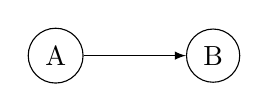
\begin{tikzpicture}
    \node[draw,circle] at (0,0) (a) {A};
    \node[draw,circle] at (2,0) (b) {B};
    \draw[->,>=latex] (a) -> (b);
  \end{tikzpicture}
  \caption[A simple graph drawing]{A simple graph drawing showing how
    to get from A to B.}
  \label{fig:atob}
\end{figure}

Images are usually included as figures as
well. Figure~\ref{fig:screenshot} shows a screenshot taken while
preparing this document.
\begin{figure}[ht]
  \centering
  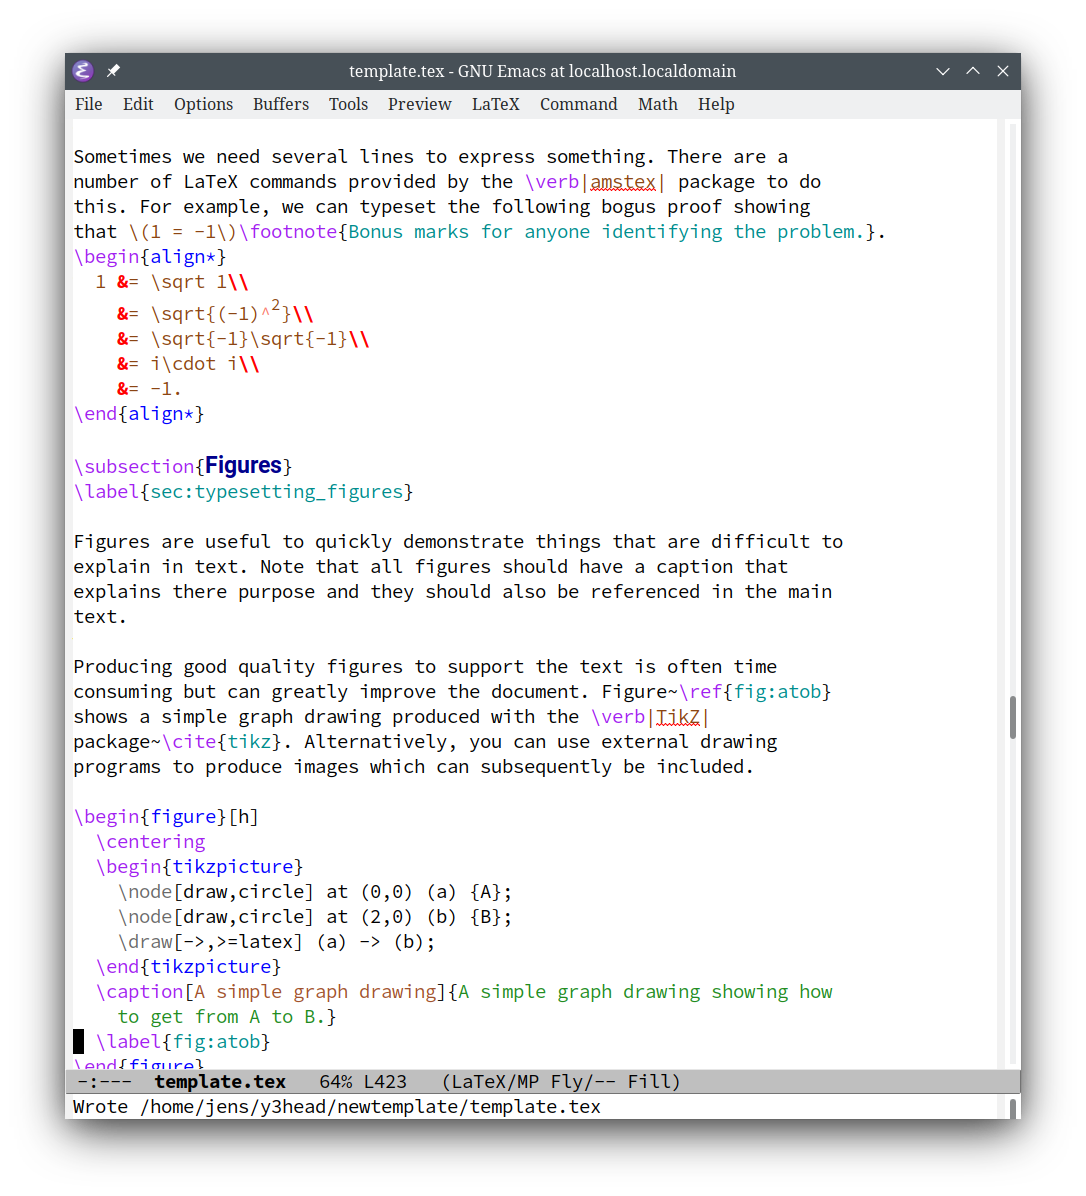
\includegraphics[width=70mm]{img/screenshot}
  \caption{Screenshot showing LaTeX document under preparation.}
  \label{fig:screenshot}
\end{figure}

\subsubsection{Avoid directly importing other peoples images}

It is best if you produce figures/images that are directly relevant to
your project rather than taking images from other people. If you do
take images from other sources these need to be cited in the caption
with an entry in the bibliography.

\subsection{Code listings}
\label{sec:typesetting_listings}

Code listings can be useful to describe key points in an
implementation. In this document we have used the \verb|listings|
package~\cite{ctan-listings}. If you desire more advanced code
highlighting then you may want to look at the \verb|minted|
package~\cite{ctan-minted}.

Code listings generally use a monospace font so characters line up
vertically.

% Long form code listings can be taken directly from an external file.
\lstinputlisting[language={c}, label={lst:c_hello_world}, caption={An
  implementation of an important algorithm from our
  work.}]{./listings/hello_world.c}

It is also possible to use code fragments inline. For example,
\lstinline[language=c]|int argc|.

\subsection{Tables}
\label{sec:typesetting_tables}

A table is a very good way to present a modest amount of data. It
should be quite clear from Table~\ref{tab:optimise} that the
optimisation really improved the running times, and also that the
improvements were better for Algorithm A than for Algorithm B. As with
figures, tables should have captions and be referenced in the text. We
have made use of the package \verb|booktabs|~\cite{ctan-booktabs} for
more pleasing results.

\begin{table}[ht]
  \centering
  \begin{tabular}{lrrrr}
    \toprule
    & \multicolumn{2}{c}{Non-optimised} & \multicolumn{2}{c}{Optimised}
    \\\cmidrule(lr){2-3}\cmidrule(lr){4-5}
    & Steps & Time (ms) & Steps  & Time (ms) \\
    \midrule
    Algorithm A & 4711 & 13.9 & 2424 & 6.9 \\
    Algorithm B & 2800 & 16.2 & 2022 & 11.2 \\
    \bottomrule
  \end{tabular}
  \caption{Reporting on some ficticious optimisation results.}
  \label{tab:optimise}
\end{table}

\section{Conclusions}
\label{sec:conclusion}

Finally, it is time to write up a summary of the things
accomplished. In our case this is a template that may be used as a
basis for your own dissertation.

You would normally also discuss future work. This might be
improvements to the project that has come to light while reflecting on
the outcomes, or it could be open questions that so far remain unanswered.

% Prints the Reference section
\printbibliography 

% Appendices are used to provide bulk information that does not fit
% into the main text. Common content is program code and data
% sets. You may want to discuss key elements in the main text, but
% provide the rest in an appendix for completeness.
\clearpage\appendix

\section{Implementation of main algorithm}
\label{app:implementation_algorithm}

% Code listings should live in a code file, not embedded directly into your LaTeX code!
\lstinputlisting[language=c, caption={An implementation of an important algorithm from our work.}]{./listings/hello_world.c}

\end{document}
